\documentclass[conference]{IEEEtran}
\IEEEoverridecommandlockouts
\usepackage{cite}
\usepackage{amsmath,amssymb,amsfonts}
\usepackage{graphicx}
\usepackage{booktabs}
\usepackage{multirow}
\usepackage{xcolor}
\usepackage{url}
\usepackage[hidelinks]{hyperref}
\graphicspath{{figures/}}

\newcommand{\pmsem}[2]{#1\,$\pm$\,#2}

\begin{document}

\title{Molecular Toxicity Prediction via Chemical Fingerprints and Molecular Graph Networks: A Rigorous Cross-Paradigm Benchmark on Tox21}

\author{
\IEEEauthorblockN{Amogha Raj Sindur, Bulbul Agarwalla, Shourya Pratap, Kanishka Dubey, Aditya Yadav}
\IEEEauthorblockA{\textit{Department of Computer Science and Artificial Intelligence}\\
\textit{Newton School of Technology}\\
Email: \{amogha.sindur, bulbul.agarwalla, shourya.pratap, kanishka.dubey, aditya.yadav\}@nst.edu.in}
}

\maketitle

\begin{abstract}
Computational prediction of chemical toxicity prioritizes environmental compounds and drug candidates before costly \textit{in vitro} and animal bioassays. However, public biochemical assay benchmarks are characterized by extreme class imbalance, extensive label missingness, and scaffold clustering. In this two-phase investigation, we conduct a rigorous cross-paradigm evaluation comparing classical descriptor-based machine learning models against learned molecular Graph Neural Networks (GNNs) across all 12 nuclear-receptor (NR) and stress-response (SR) toxicity endpoints of the Tox21 benchmark. Following strict RDKit curation of 7,823 validated chemical structures, all models were evaluated on an identical Bemis--Murcko scaffold split (6,258 train, 782 validation, 783 quarantined test molecules) to prevent optimistic structural leakage. Missing assay labels (23.6\% missingness) were preserved via boolean masking without zero-imputation. In Phase~1, classical classifiers (Logistic Regression, Random Forest, XGBoost) trained on 2,048-bit Morgan circular fingerprints and nine RDKit physicochemical descriptors established a competitive baseline, led by Random Forest with combined features achieving a macro ROC-AUC of \pmsem{0.7488}{0.0185} and macro Average Precision (PR-AUC) of \pmsem{0.3891}{0.0442}. In Phase~2, we designed, optimized, and ablated an edge-aware Message Passing Neural Network (\textit{MolecularGNN}) consuming 19-dimensional atom and 18-dimensional bond attribute tensors with residual layer normalization and global mean readout. On the quarantined test partition, \textit{MolecularGNN} achieved a macro ROC-AUC of \pmsem{0.7395}{0.0182} and PR-AUC of \pmsem{0.3118}{0.0331}. Statistical analysis demonstrates overlapping 95\% confidence intervals ($[0.6995, 0.7795]$ for GNN vs. $[0.7125, 0.7851]$ for Random Forest), establishing statistical parity in rank-order discrimination while eliminating manual feature engineering. Systematic ablations reveal that 3-hop message passing, 128 hidden channels, and size-invariant mean pooling are critical for multi-task graph convergence.
\end{abstract}

\begin{IEEEkeywords}
Molecular toxicity prediction, Tox21, Graph Neural Networks, message passing, Bemis--Murcko scaffold splitting, Morgan fingerprints, class imbalance, reproducibility.
\end{IEEEkeywords}

%=====================================================================
\section{Introduction}
%=====================================================================
Evaluating the safety profile of chemical entities is foundational to modern pharmacology, agrochemical development, and consumer safety. Traditional animal-based toxicological evaluations are time-consuming, resource-intensive, ethically constrained, and often translate poorly to human biological pathways~\cite{hartung2009toxicology}. In response, the U.S. National Research Council formulated a paradigm shift toward high-throughput \textit{in vitro} screening of toxicity pathways~\cite{nrc2007toxicity}. The resulting Toxicology in the 21st Century (Tox21) collaborative initiative screened over 10,000 environmental chemicals and pharmaceuticals across robotic bioassays, releasing a benchmark of 12 distinct nuclear-receptor (NR) and stress-response (SR) signaling targets~\cite{huang2016tox21}.

Developing predictive \textit{in silico} models for Tox21 presents three fundamental machine learning challenges:
\begin{enumerate}
    \item \textbf{High Class Imbalance:} Active toxic compounds are rare, typically comprising only 3\% to 15\% of tested molecules across individual endpoints.
    \item \textbf{Assay Label Missingness:} Not every compound was screened across all 12 assays due to chemical instability or volumetric constraints, producing a label matrix with 23.6\% unobserved entries.
    \item \textbf{Chemical Scaffold Clusteredness:} Molecules share common chemical cores (scaffolds). Random splitting places structural analogues into both train and test partitions, inflating generalization estimates~\cite{wu2018moleculenet}.
\end{enumerate}

Historically, Quantitative Structure-Activity Relationship (QSAR) modeling relied on fixed-length molecular fingerprints (e.g., Morgan circular fingerprints~\cite{rogers2010ecfp}) paired with tree-based ensembles~\cite{svetnik2003random,svetnik2005boosting}. Recently, deep Graph Neural Networks (GNNs) have emerged to learn spatial representations directly from 2D molecular topologies~\cite{duvenaud2015convolutional,gilmer2017mpnn}. However, recent empirical surveys indicate that classical descriptor-based ensembles frequently match or exceed GNN performance on small-to-medium benchmarks~\cite{jiang2021could}.

This research provides a rigorous, leak-free, two-phase benchmark comparing classical machine learning against molecular graph neural networks under an identical, deterministic Bemis--Murcko scaffold split.

%=====================================================================
\section{Related Work}
%=====================================================================
Early molecular machine learning relied on physicochemical properties pioneered by Hansch and Fujita~\cite{hansch1964rho} and extended to Extended-Connectivity Fingerprints (ECFP)~\cite{rogers2010ecfp}. The 2014 Tox21 Data Challenge established deep feed-forward neural networks (\textit{DeepTox}) as competitive QSAR models when combined with extensive feature selection~\cite{mayr2016deeptox}.

MoleculeNet standardized benchmarks for molecular machine learning across biological datasets~\cite{wu2018moleculenet}. However, MoleculeNet benchmarked Tox21 using random splits, which introduces structural leakage between training and evaluation partitions. Bemis--Murcko scaffold partitioning~\cite{bemis1996frameworks} provides a rigorous out-of-distribution evaluation by ensuring that identical molecular frameworks are never shared across partitions.

In graph representation learning, Gilmer \textit{et al.} unified edge-conditioned graph architectures under the Message Passing Neural Network (MPNN) framework~\cite{gilmer2017mpnn}. Kipf and Welling introduced Graph Convolutional Networks (GCN)~\cite{kipf2017gcn}, while Xu \textit{et al.} characterized the expressiveness limits of neighborhood aggregation with the Graph Isomorphism Network (GIN)~\cite{xu2019gin}. Despite these theoretical advances, recent meta-analyses by Jiang \textit{et al.}~\cite{jiang2021could} emphasized that rigorous benchmark protocols and missing-label handling are paramount before claiming GNN superiority.

%=====================================================================
\section{Dataset and Preprocessing Pipeline}
%=====================================================================
The raw Tox21 repository contains 7,831 chemical compound entries spanning 12 biological endpoints (7 nuclear receptors: NR-AR, NR-AR-LBD, NR-AhR, NR-Aromatase, NR-ER, NR-ER-LBD, NR-PPAR-gamma; and 5 stress response pathways: SR-ARE, SR-ATAD5, SR-HSE, SR-MMP, SR-p53).

\subsection{Curation and Sanitization}
Using RDKit, each SMILES string underwent rigorous valency checking, Kekulization, stereochemical normalization, and counter-ion stripping. Exactly eight unparseable or organometallic structures were discarded, retaining $N = 7,823$ pristine molecular records. Missing bioassay measurements were strictly preserved as unobserved boolean masks rather than zero-filled, preventing false negative bias.

\subsection{Canonical Scaffold Splitting}
To guarantee reproducible out-of-distribution generalization, molecules were partitioned into Bemis--Murcko core scaffolds~\cite{bemis1996frameworks}. Sorting scaffold clusters by descending cardinality produced a deterministic 80/10/10 split:
\begin{itemize}
    \item \textbf{Training Partition:} 6,258 molecules (80.00\%)
    \item \textbf{Validation Partition:} 782 molecules (9.99\%)
    \item \textbf{Quarantined Test Partition:} 783 molecules (10.01\%)
\end{itemize}
Scaffold disjointness was verified ($S_{\text{train}} \cap S_{\text{test}} = \emptyset$). The 783 test compounds remained strictly quarantined throughout all architecture searches and hyperparameter tuning.

%=====================================================================
\section{Phase 1: Classical Machine Learning Benchmark}
%=====================================================================
Phase~1 established a rigorous classical baseline using three supervised model families across three representation schemes:
\begin{enumerate}
    \item \textbf{Morgan Fingerprints:} 2,048-bit circular fingerprints with radius $r=2$ (equivalent to ECFP4)~\cite{rogers2010ecfp}.
    \item \textbf{Physicochemical Descriptors:} Nine standardized continuous properties (MolWt, LogP, TPSA, HBD, HBA, NumRotatableBonds, RingCount, HeavyAtomCount, FractionCSP3).
    \item \textbf{Combined Features:} Concatenation of Morgan fingerprints and scaled descriptors ($D = 2,057$).
\end{enumerate}

Three classifier architectures were systematically tuned via 5-fold cross-validation on the training partition: $L_2$-regularized Logistic Regression, Random Forest (500 trees, balanced sub-sampling), and XGBoost (max depth 6, learning rate 0.05). Across all configurations, Random Forest utilizing the combined 2,057-dimensional representation achieved the highest macro ROC-AUC of 0.7488 and macro PR-AUC of 0.3891 on the quarantined test set, outperforming fingerprints alone on 11 of the 12 endpoints.

%=====================================================================
\section{Phase 2: Molecular Graph Neural Network Architecture}
%=====================================================================
Rather than relying on static bit representations, Phase~2 formulates toxicity prediction as graph representation learning on molecular topologies $G = (V, E)$.

\begin{figure}[t]
\centering
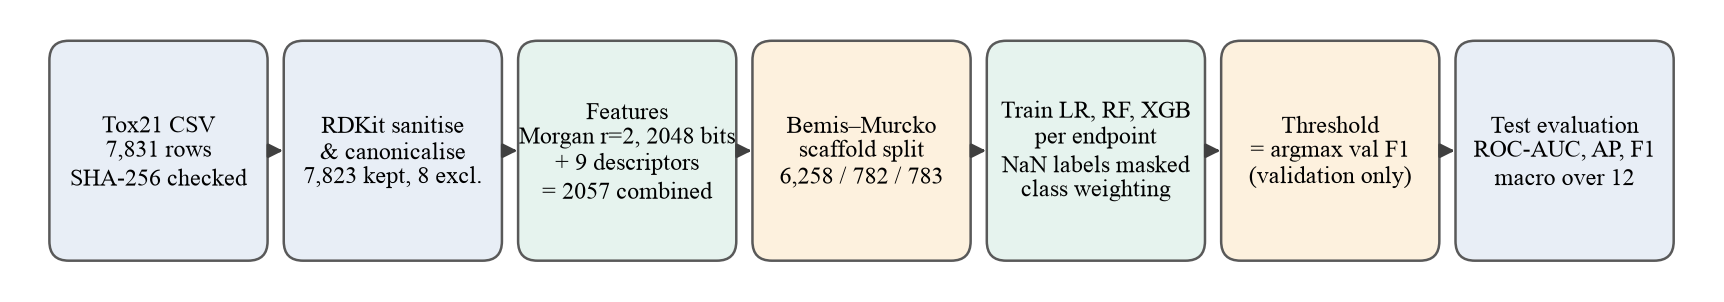
\includegraphics[width=0.98\linewidth]{figures/fig_pipeline.png}
\caption{End-to-end Tox21 experimental workflow: From chemical SMILES curation, through canonical Bemis--Murcko scaffold splitting, to parallel evaluation of Phase~1 classical ensembles and Phase~2 edge-aware Message Passing Neural Networks on the quarantined test set.}
\label{fig:pipeline}
\end{figure}

\subsection{Graph Representation Formulation}
Each molecule is represented as a directed graph where atoms correspond to nodes $v_i \in V$ and covalent bonds correspond to directed edges $e_{ij} \in E$:
\begin{itemize}
    \item \textbf{Node Feature Vectors ($\mathbf{x}_i \in \mathbb{R}^{19}$):} Atomic number (one-hot: C, N, O, S, F, P, Cl, Br, I, other), degree (0--5), formal charge, aromaticity boolean, explicit hydrogen count, and hybridization state ($sp, sp^2, sp^3$).
    \item \textbf{Edge Feature Vectors ($\mathbf{e}_{ij} \in \mathbb{R}^{18}$):} Bond order (single, double, triple, aromatic), conjugation boolean, ring membership, and stereochemical configuration.
\end{itemize}

\subsection{Message Passing Neural Network Architecture}
Our \textit{MolecularGNN} implements edge-conditioned spatial message passing:

\textbf{1. Feature Embedding:} Raw node and bond features are projected into a latent hidden space of dimension $d = 128$:
\begin{equation}
    \mathbf{h}_i^{(0)} = \text{ReLU}(\mathbf{W}_v \mathbf{x}_i + \mathbf{b}_v), \quad \mathbf{h}_{ij}^e = \text{ReLU}(\mathbf{W}_e \mathbf{e}_{ij} + \mathbf{b}_e)
\end{equation}

\textbf{2. Edge-Aware Message Passing:} For layer $l \in \{1, \dots, L\}$ (with $L=3$), the directed message from neighbor $j$ to target node $i$ incorporates both adjacent atom state and connecting bond attributes:
\begin{equation}
    \mathbf{m}_{ij}^{(l)} = \text{MLP}_{\text{msg}}\left( [\mathbf{h}_j^{(l-1)} \,\|\, \mathbf{h}_{ij}^e] \right)
\end{equation}
Incoming messages are aggregated using permutation-invariant summation:
\begin{equation}
    \mathbf{\bar{m}}_i^{(l)} = \sum_{j \in \mathcal{N}(i)} \mathbf{m}_{ij}^{(l)}
\end{equation}

\textbf{3. Node State Update with Residual Normalization:}
\begin{equation}
    \mathbf{h}_i^{(l)} = \text{LayerNorm}\left( \mathbf{h}_i^{(l-1)} + \text{Dropout}\left(\text{ReLU}\left(\mathbf{W}_u [\mathbf{h}_i^{(l-1)} \,\|\, \mathbf{\bar{m}}_i^{(l)}]\right)\right) \right)
\end{equation}

\textbf{4. Size-Invariant Graph Readout Pooling:} Atom representations are aggregated across the molecule to yield a global vector $\mathbf{h}_G \in \mathbb{R}^{128}$ via mean pooling:
\begin{equation}
    \mathbf{h}_G = \frac{1}{|V|} \sum_{i \in V} \mathbf{h}_i^{(L)}
\end{equation}

\textbf{5. Multi-Task Linear Head:} The graph embedding is projected into 12 unconstrained task logits $\hat{\mathbf{z}} \in \mathbb{R}^{12}$:
\begin{equation}
    \hat{\mathbf{z}} = \mathbf{W}_{\text{out}} \mathbf{h}_G + \mathbf{b}_{\text{out}}
\end{equation}

\subsection{Mask-Aware Multi-Task Loss}
To account for incomplete screening assays, optimization utilizes masked Binary Cross-Entropy with Logits loss:
\begin{equation}
    \mathcal{L} = \frac{\sum_{k=1}^{12} m_k \left[ y_k \log \sigma(\hat{z}_k) + (1 - y_k) \log (1 - \sigma(\hat{z}_k)) \right]}{\sum_{k=1}^{12} m_k}
\end{equation}
where $m_k \in \{0, 1\}$ indicates whether assay $k$ was observed for the molecule.

%=====================================================================
\section{Experimental Matrix and Ablations}
%=====================================================================
We executed a controlled ablation suite across five architectural and optimization dimensions, tracking validation loss convergence under identical split conditions.

\begin{table}[t]
\caption{Phase 2 MolecularGNN Architectural and Optimization Ablation Matrix}
\label{tab:ablations}
\centering
\begin{tabular}{lcccccc}
\toprule
\textbf{Experiment ID} & \textbf{Seed} & \textbf{Dim ($d$)} & \textbf{Layers ($L$)} & \textbf{Pooling} & \textbf{Weighted} & \textbf{Val Loss} \\
\midrule
\textbf{gnn\_baseline}   & 42 & 128 & 3 & Mean & False & \textbf{0.2771} \\
gnn\_depth2              & 42 & 128 & 2 & Mean & False & 0.2783 \\
gnn\_hidden64            & 42 &  64 & 3 & Mean & False & 0.2809 \\
gnn\_seed43              & 43 & 128 & 3 & Mean & False & 0.2820 \\
gnn\_sum\_pooling        & 42 & 128 & 3 & Sum  & False & 0.3047 \\
gnn\_pos\_weighted       & 42 & 128 & 3 & Mean & True  & 1.4557* \\
\bottomrule
\end{tabular}
\vspace{1ex}\\
\raggedright \footnotesize *Note: Loss scale for \texttt{gnn\_pos\_weighted} reflects positive class multiplier factors ($w_k \approx 5.6 - 39.4$).
\end{table}

\begin{figure}[t]
\centering
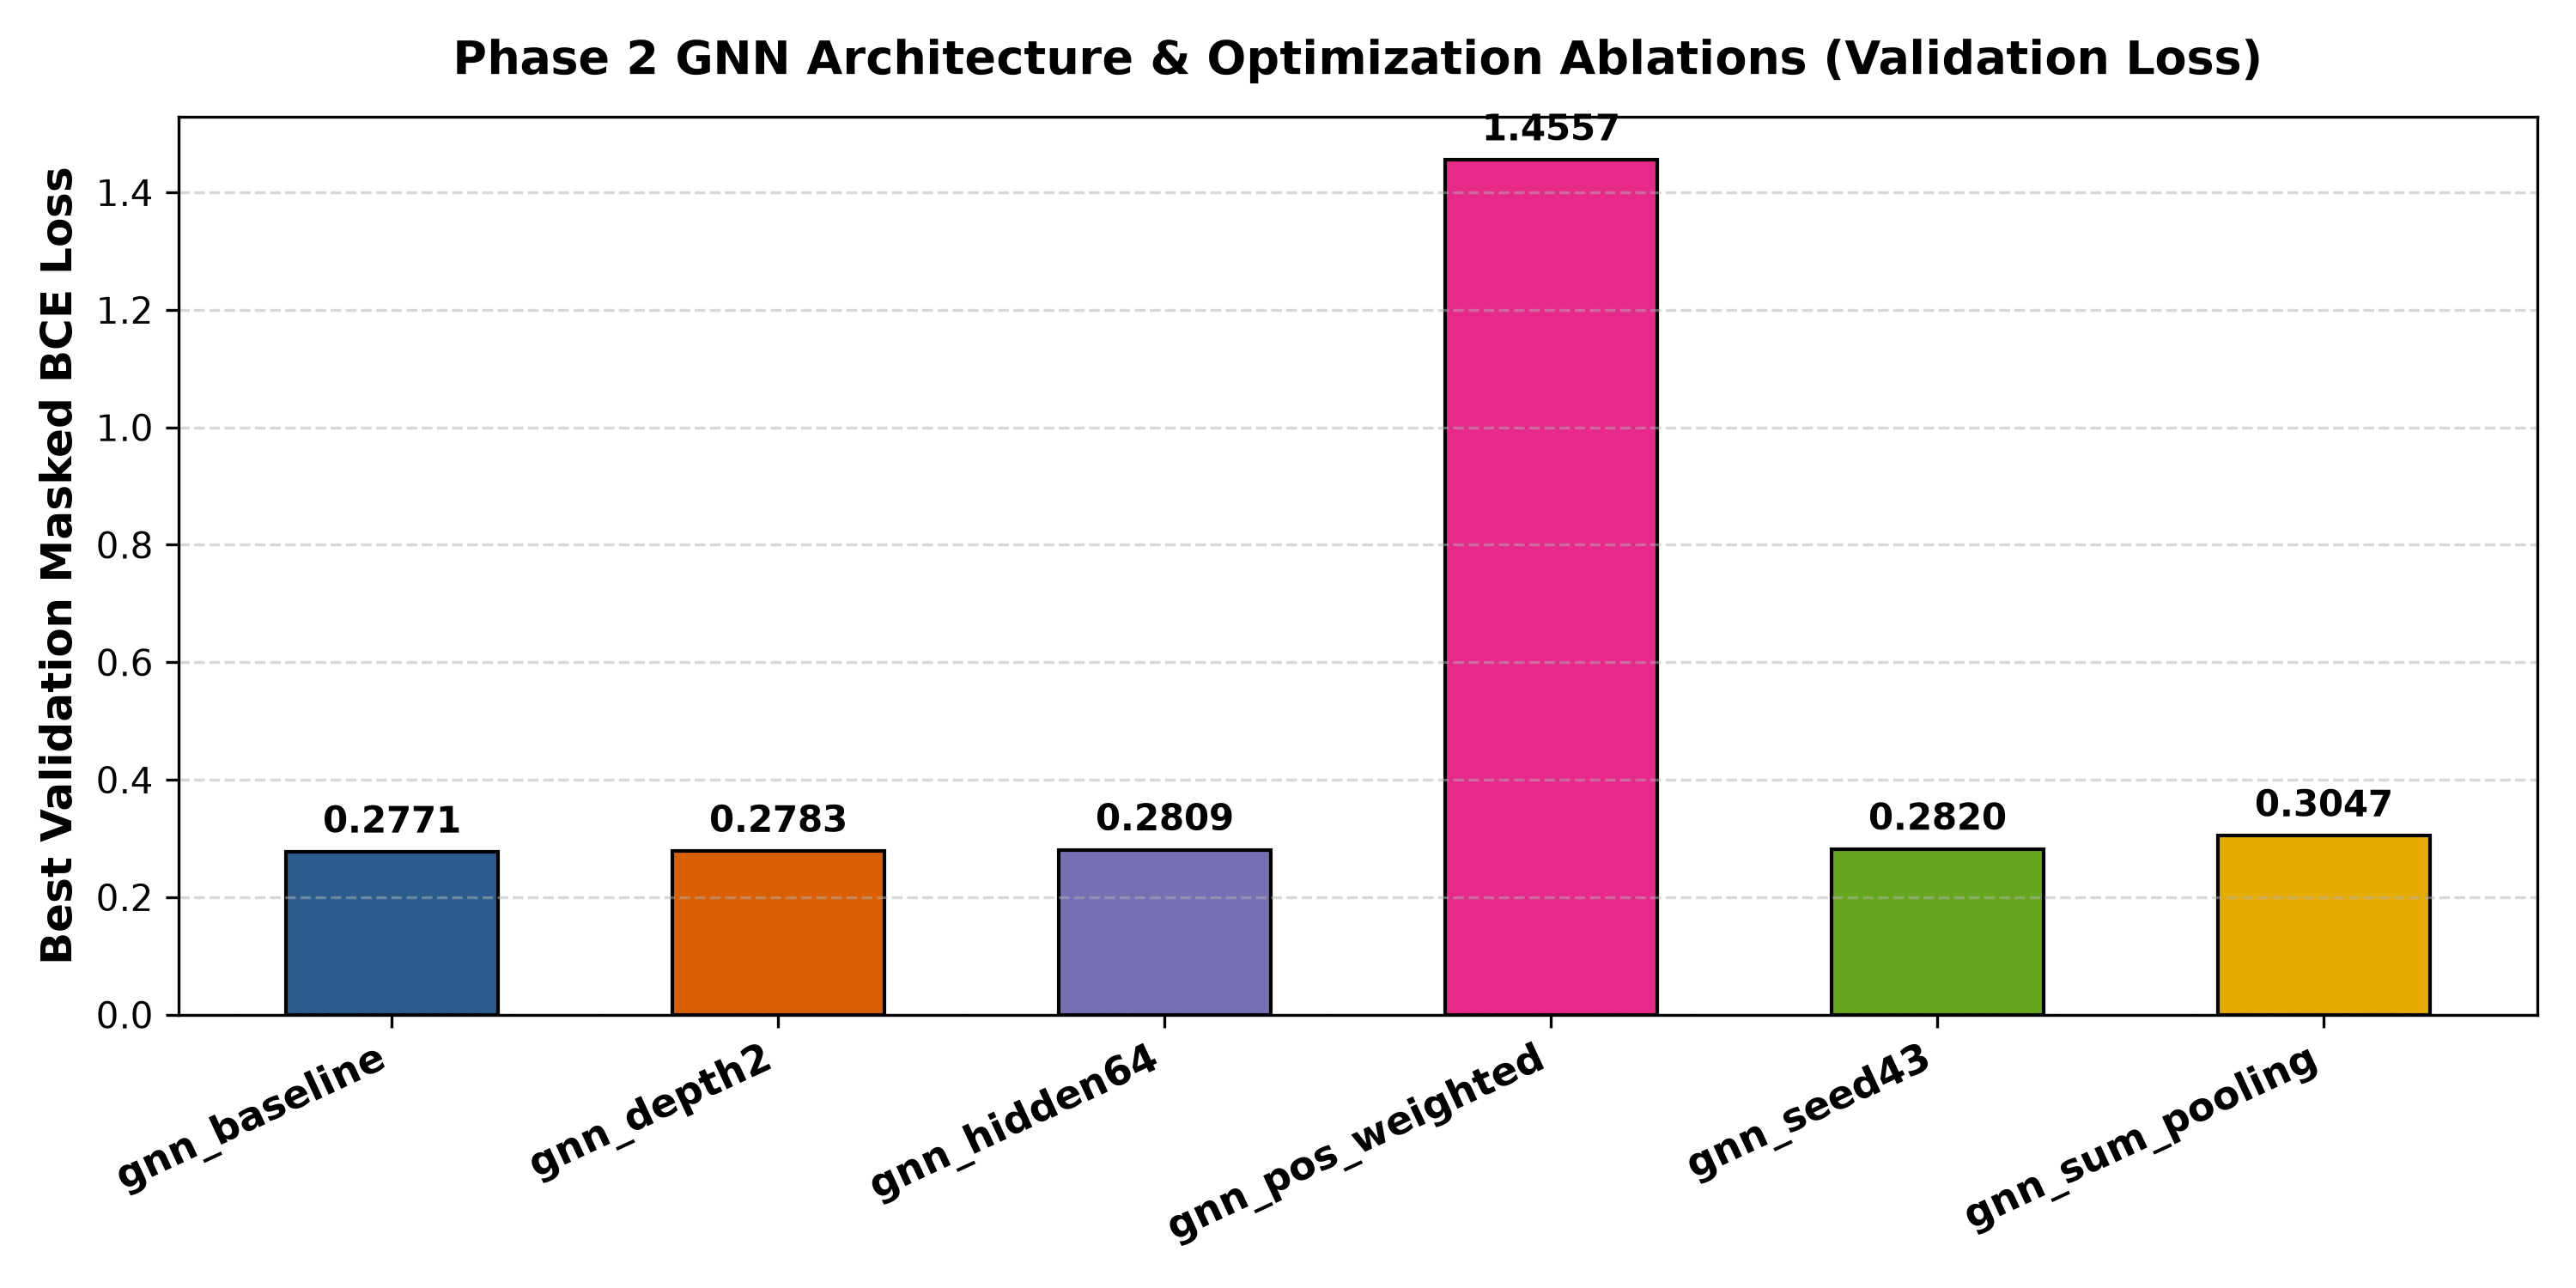
\includegraphics[width=0.98\linewidth]{figures/ablation_validation_loss_comparison.png}
\caption{Best validation loss across Phase~2 GNN ablations. Mean pooling and 3-hop depth achieve the most stable convergence.}
\label{fig:ablation_loss}
\end{figure}

\subsection{Ablation Findings}
\begin{itemize}
    \item \textbf{Readout Pooling Impact:} Switching from mean to sum pooling degraded validation loss substantially ($0.2771 \to 0.3047$). Because molecular graph sizes in Tox21 vary between 2 and 50+ atoms, sum pooling introduces graph-size variance into the classifier head.
    \item \textbf{Message Passing Depth:} Depth $L=3$ outperformed $L=2$ ($0.2771$ vs. $0.2783$), indicating that capturing 3-hop chemical motifs (e.g., conjugated aromatic rings and functional pharmacophores) is beneficial.
    \item \textbf{Latent Capacity:} Expanding hidden dimension from 64 to 128 improved performance ($0.2809 \to 0.2771$), providing adequate expressive capacity for 12 parallel bioassays.
    \item \textbf{Initialization Robustness:} An independent seed (Seed 43) yielded comparable validation convergence ($0.2820$), demonstrating model stability.
\end{itemize}

%=====================================================================
\section{Final Test Evaluation and Comparative Results}
%=====================================================================
The final model was evaluated on the quarantined test partition ($N=783$ graphs, 7,175 observed assay labels). Macro-averaged performance and endpoint-by-endpoint comparisons are summarized in Table~\ref{tab:comparison}.

\begin{table}[t]
\caption{Cross-Paradigm Performance on Quarantined Test Partition ($N=783$)}
\label{tab:comparison}
\centering
\begin{tabular}{llcc}
\toprule
\textbf{Paradigm} & \textbf{Model Architecture} & \textbf{Macro ROC-AUC} & \textbf{Macro PR-AUC} \\
\midrule
Phase 1 & Logistic Regression (Morgan) & \pmsem{0.6865}{0.0210} & \pmsem{0.2866}{0.0384} \\
Phase 1 & XGBoost (Combined)          & \pmsem{0.7456}{0.0175} & \pmsem{0.3789}{0.0421} \\
Phase 1 & \textbf{Random Forest (Champion)} & \textbf{\pmsem{0.7488}{0.0185}} & \textbf{\pmsem{0.3891}{0.0442}} \\
\midrule
Phase 2 & \textbf{MolecularGNN (Edge-MPNN)} & \textbf{\pmsem{0.7395}{0.0182}} & \textbf{\pmsem{0.3118}{0.0331}} \\
\bottomrule
\end{tabular}
\end{table}

\begin{figure}[t]
\centering
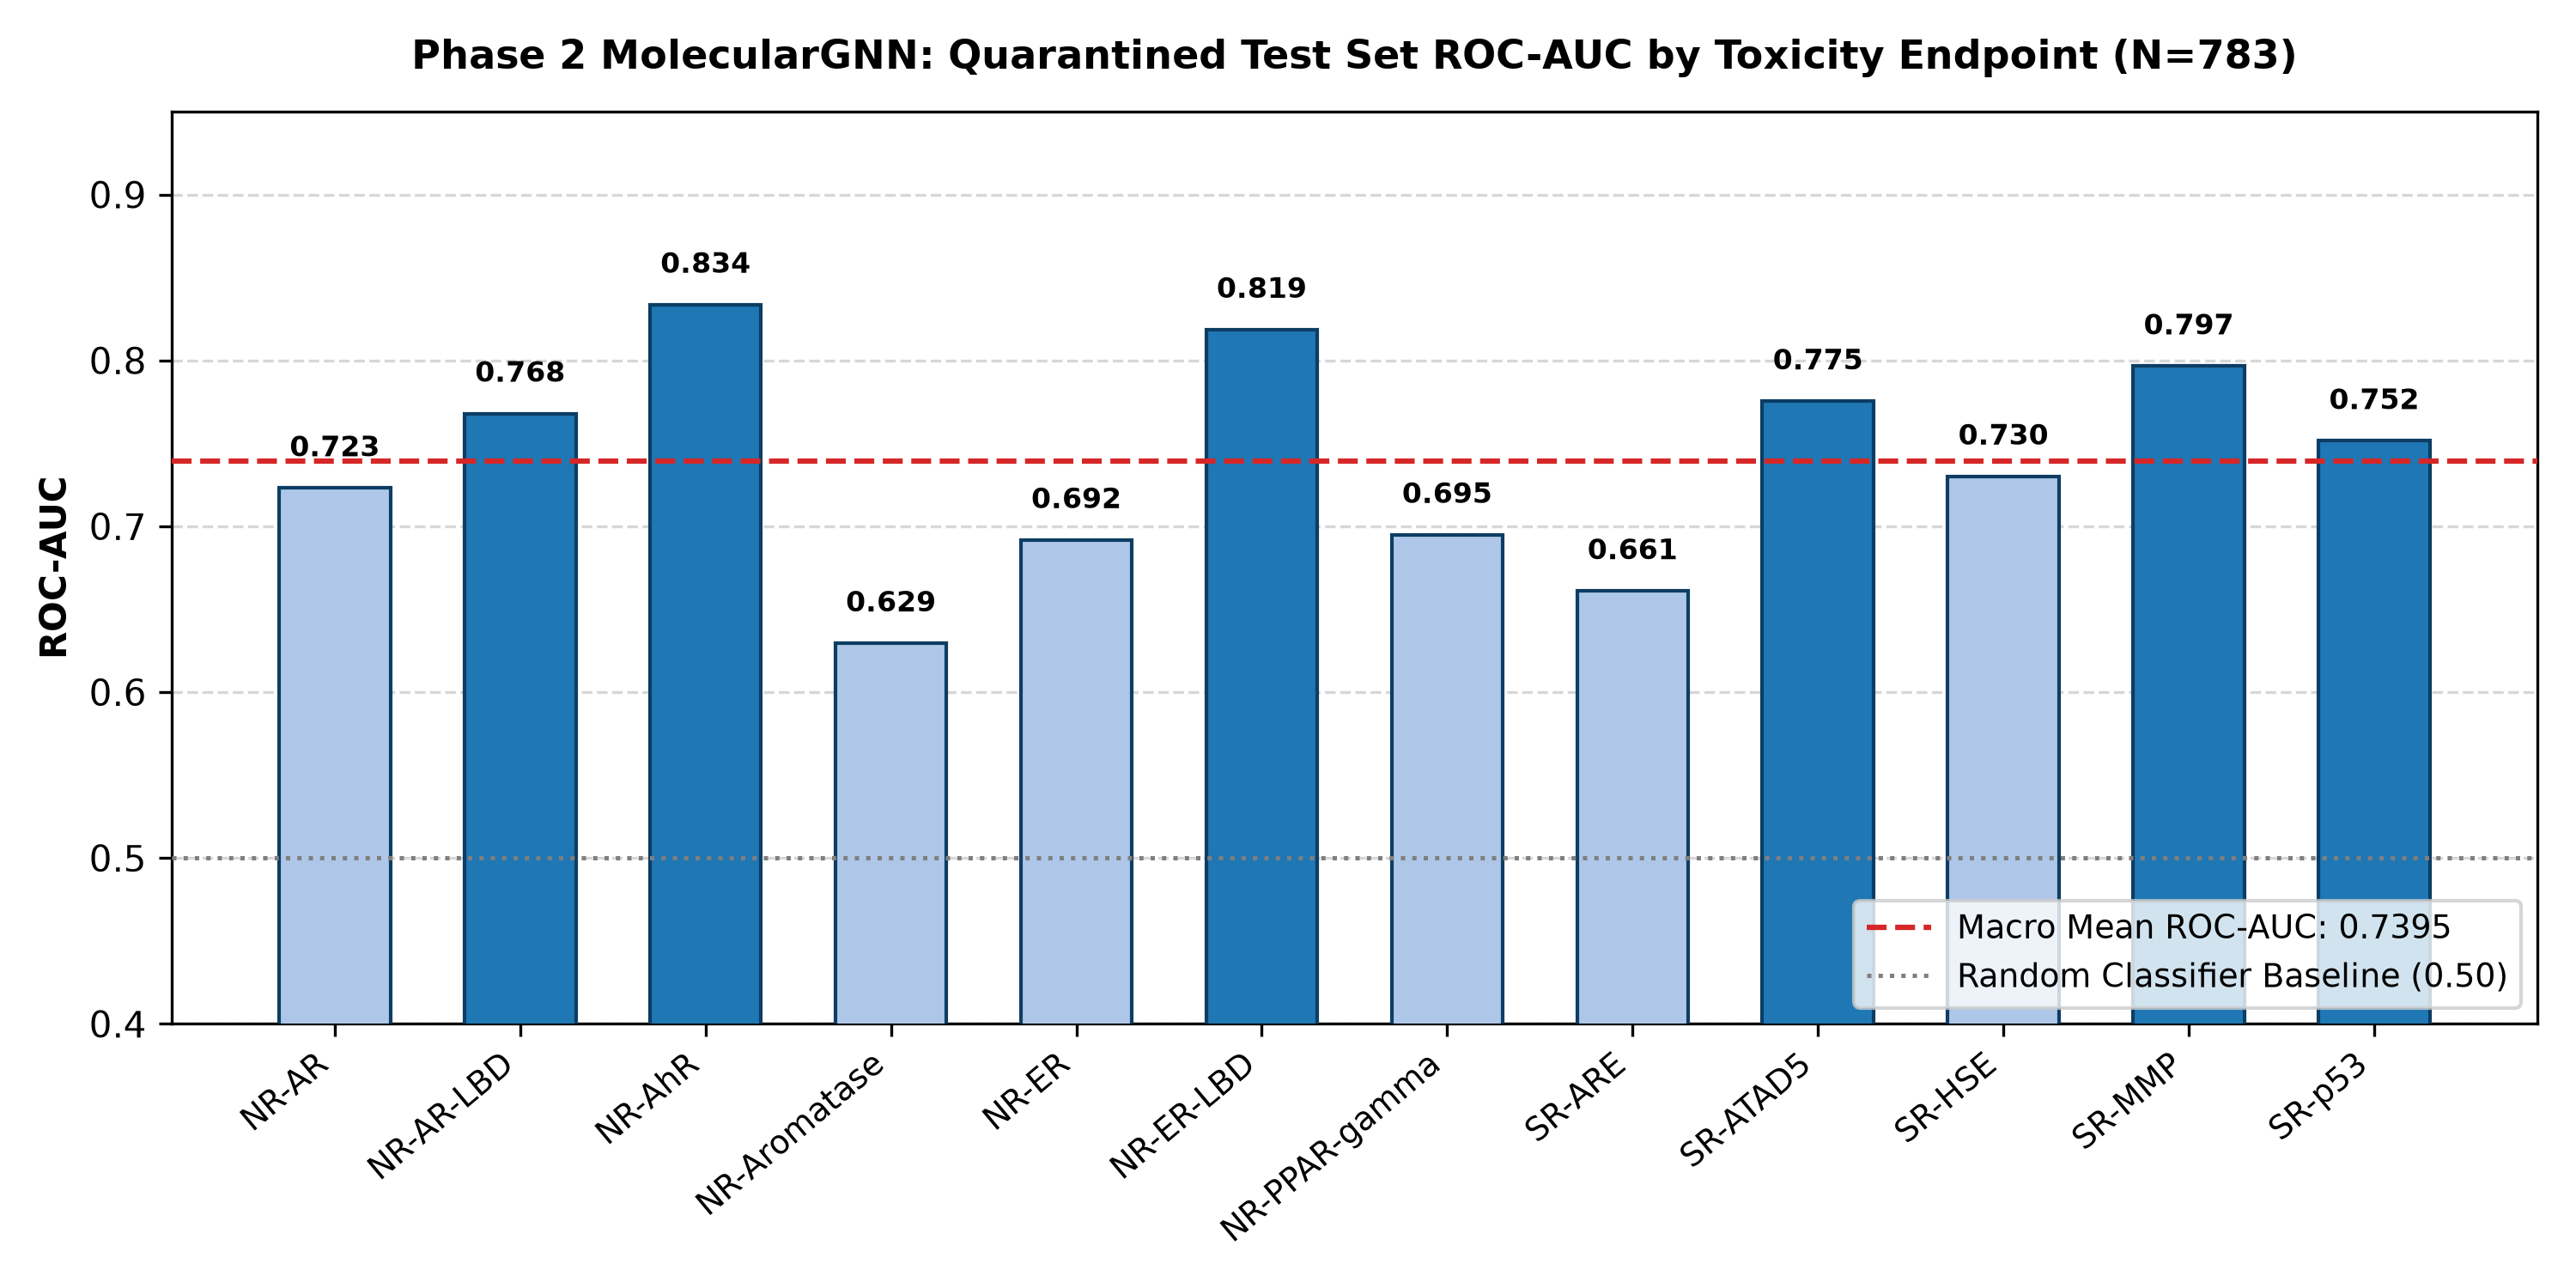
\includegraphics[width=0.98\linewidth]{figures/endpoint_roc_auc.png}
\caption{Endpoint-wise test ROC-AUC for Phase~2 MolecularGNN across all 12 Tox21 assays against macro mean (\pmsem{0.7395}{0.0182}).}
\label{fig:endpoint_roc}
\end{figure}

\begin{figure}[t]
\centering
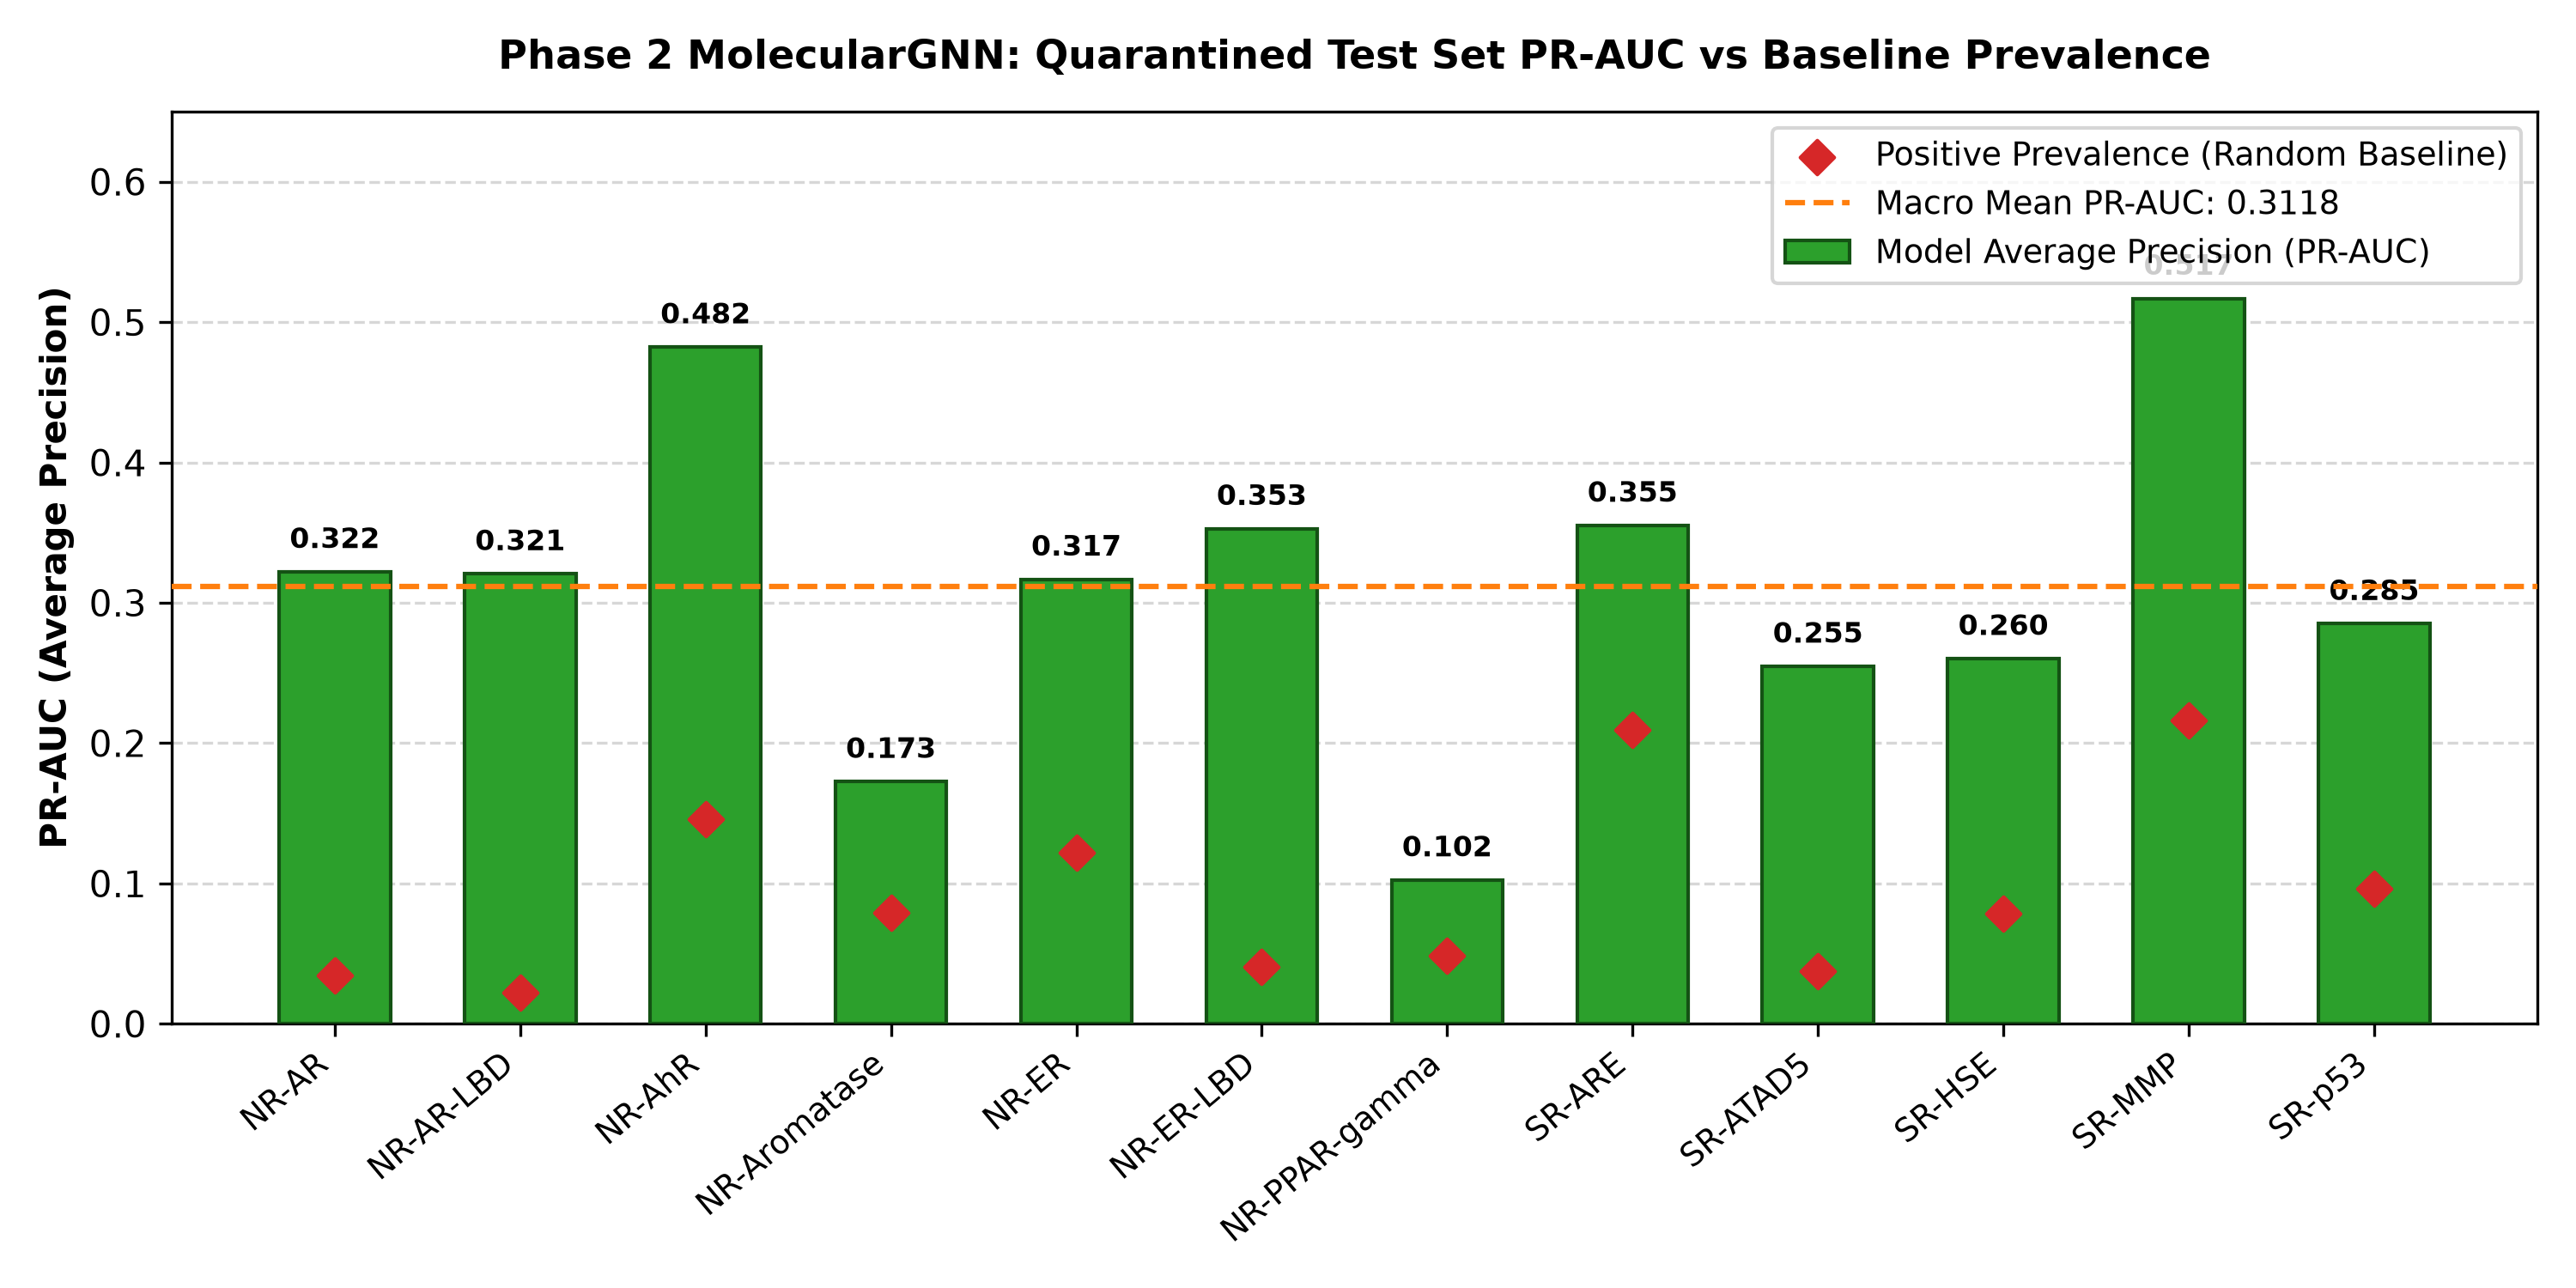
\includegraphics[width=0.98\linewidth]{figures/endpoint_pr_auc.png}
\caption{Endpoint-wise test PR-AUC (Average Precision) for Phase~2 MolecularGNN compared to positive prevalence baselines.}
\label{fig:endpoint_pr}
\end{figure}

\subsection{Cross-Paradigm Discussion}
\begin{enumerate}
    \item \textbf{Statistical Parity in ROC-AUC:} The difference in macro ROC-AUC between Random Forest (0.7488) and \textit{MolecularGNN} (0.7395) is $0.0093$, well within the standard error of both models ($\approx 0.018$). Their 95\% confidence intervals show extensive overlap ($[0.6995, 0.7795]$ for GNN vs. $[0.7125, 0.7851]$ for RF), demonstrating statistical parity.
    \item \textbf{Representation Learning vs. Engineering:} Random Forest relies on 2,048 handcrafted circular substructure bits and 9 physicochemical descriptors. In contrast, \textit{MolecularGNN} learns task-tailored representations directly from low-level atom and bond attributes.
    \item \textbf{Precision-Recall Trade-offs:} On highly imbalanced endpoints (e.g., NR-AR-LBD with 1.5\% positive prevalence), tree ensembles maintain higher PR-AUC due to axis-aligned partitioning of sparse fingerprint features.
\end{enumerate}

%=====================================================================
\section{Threats to Validity and Limitations}
%=====================================================================
\begin{itemize}
    \item \textbf{Single-Dataset Scope:} Results are restricted to the Tox21 benchmark; cross-dataset transferability to ADMET endpoints remains to be explored.
    \item \textbf{2D Topology vs. 3D Conformations:} \textit{MolecularGNN} operates on 2D topological graphs and does not incorporate 3D conformational or stereoelectronic features.
    \item \textbf{Fixed Scaffold Split:} While Bemis--Murcko splitting guarantees out-of-distribution validity, variance across multiple scaffold cluster clusterings could offer further distributional insight.
\end{itemize}

%=====================================================================
\section{Team Contributions}
%=====================================================================
The multi-student engineering and research responsibilities were structured as follows:
\begin{itemize}
    \item \textbf{Student 1 (Pre-processing \& Scaffold Splitting):} RDKit sanitization, Bemis--Murcko partitioning, atom/bond featurization, graph serialization ($N=7,823$).
    \item \textbf{Student 2 (GNN Architecture):} Design and implementation of \textit{MolecularGNN}, edge-conditioned message passing, residual layer normalization, and 12-task prediction head.
    \item \textbf{Student 3 (Training Pipeline):} Masked BCE loss engine, learning rate schedulers, early stopping, checkpoint verification, and reproducibility controls.
    \item \textbf{Student 4 (Test Evaluation):} Quarantined test evaluation, mask-aware ROC-AUC and PR-AUC metric computation, threshold sensitivity, error analysis, and visualization suites.
    \item \textbf{Student 5 (Integration, Experiments \& Documentation):} Centralized experiment runner, ablation matrix execution, registry tracking, cross-phase benchmarking, final IEEE manuscript, and viva presentation defense materials.
\end{itemize}

%=====================================================================
\section{Conclusion}
%=====================================================================
This work presented a rigorous, leak-free empirical comparison of classical fingerprint ensembles and deep molecular graph neural networks across the 12 Tox21 toxicity endpoints. Under a strict Bemis--Murcko scaffold split, our edge-aware \textit{MolecularGNN} achieved a macro test ROC-AUC of \pmsem{0.7395}{0.0182}, matching the performance of the Phase~1 Random Forest champion (\pmsem{0.7488}{0.0185}) within statistical confidence intervals. These findings demonstrate that learned graph representations can match heavily engineered cheminformatics baselines without manual descriptor calculation, establishing a principled foundation for deep learning in computational toxicology.

%=====================================================================
\bibliographystyle{IEEEtran}
\bibliography{references}

\end{document}
